\documentclass[conference]{IEEEtran}
\IEEEoverridecommandlockouts
% The preceding line is only needed to identify funding in the first footnote. If that is unneeded, please comment it out.
\usepackage{cite}
\usepackage{amsmath,amssymb,amsfonts}
\usepackage{algorithmic}
\usepackage{framed}
\usepackage{mdframed}
\usepackage{graphicx}
\usepackage{float}
\usepackage{textcomp}
\usepackage{xcolor}
\usepackage{graphicx}
\usepackage{url}
\usepackage{listings}
\usepackage{titlesec}



\def\BibTeX{{\rm B\kern-.05em{\sc i\kern-.025em b}\kern-.08em
    T\kern-.1667em\lower.7ex\hbox{E}\kern-.125emX}}


\titleformat{\subsubsubsubsection}
{\normalfont\normalsize\bfseries}{\thesubsubsubsubsection}{1em}{}
\titlespacing*{\subsubsubsubsection}{0pt}{3.25ex plus 1ex minus .2ex}{1.5ex plus .2ex}


\titlespacing{\subsection}{0pt}{\parskip}{-\parskip}

\newcommand{\subsubsubsection}[1]{\paragraph{#1}\mbox{}\\} % Define subsubsubsection command

\lstset{
  basicstyle=\ttfamily, % Set the font size to small
  % Other listing options...
}


\graphicspath{ {./} }
\begin{document}

\title{How does the use of GPUs in HPC accelerate scientific research such as deep learning and weather forecasting?
}

\author{\IEEEauthorblockN{Selim Mert Kastan}
\and
\IEEEauthorblockN{Dominik Schwarz}}

\maketitle

\begin{abstract}
Graphics Processing Units (GPUs) have emerged as powerful accelerators for complex computations. With their immense parallel processing capabilities, GPUs have revolutionized scientific research and applications. This paper explores the significance of GPUs within the High-Performance Computing (HPC) ecosystem, focusing on their utilization in training  Deep Learning and Weather models. The paper discusses GPU architecture, its operation, programming tools, and hardware advancements while comparing it to CPU technologies. 

\end{abstract}

\begin{IEEEkeywords}
GPU Acceleration, High-Performance Computing, , Deep Learning, Weather Forecasting.
\end{IEEEkeywords}

\section{Introduction}
The use of computers has enabled the scientific community to make ground-breaking discoveries and advancements. By combining massive amounts of CPUs, immense processing power in the form of supercomputers could be assembled to compute complex calculations. However, this steady climb in computational power has come to a bottleneck, as the scaling of CPU-based systems became increasingly challenging and inefficient in tackling the growing complexity of problems. Therefore, scientists were forced to find an alternative solution to this problem to cope with the ever-getting complex problems. In the early 2000s, researchers discovered  GPU-based approaches that were faster than the CPU-based approaches for the solution of general linear algebra problems. 

This realization opened up new possibilities for accelerating computations.
 In 2007, NVIDIA released CUDA, a programming platform that allowed programmers to easily adapt their codes to be compatible with GPUs. 
This innovation caused a substantial movement toward the use of GPUs, resulting in a broad acceptance and a huge influx of scientific calculations into the GPU world. \cite{b3} \cite{b26}


GPU acceleration plays an important role in scientific research, particularly in the field of artificial intelligence (AI). 
 One notable application of GPU acceleration is the development of large language models, such as GPT-3/4 by OpenAI, LLaMa by Meta, and PaLM by Google. These models contribute to widespread interactions between the masses and artificial intelligence, as Meta made its model open-source and chatbots such as ChatGPT and Bard were made available to public use, which engage in conversation and provide human-like responses to text inputs. \cite{b19}
 \cite{b20}


Furthermore, another use case is Deep learning (DL), a method of machine learning based on artificial neural networks (ANN) with representation learning. Inspired by biological systems, ANNs were trained on massive data sets to make it learn the connection between the input and output, thus making 
accurate predictions on new input data. Because of the high amounts of data that needs to be processed, HPC systems are needed to handle all of that, thus accelerating the necessary training time for Deep Learning models. This is why many of these applications use GPUs in HPC.



Another scientific area where GPUs are extensively used is weather forecasting. Weather forecasting plays a crucial role in numerous industries such as disaster management, transportation, agriculture, renewable energy, aviation, tourism, and more, as they heavily rely on accurate weather information.

To forecast weather, massive amounts of data are regularly collected from satellites in orbit and various sensors that measure temperature, atmospheric pressure, and other meteorological parameters. After the data accumulation, complex mathematical models are required to simulate various things such as atmospheric dynamics, cloud formation, precipitation patterns, and other weather phenomena, thus the need for immense computational processing power is needed, as the gathered data is too huge for a normal computer to handle in a reasonable timeframe. Therefore, computations are accelerated through parallelization with GPUs in HPC systems to provide faster and real-time results to people. \cite{b21}


In summary, the use of Graphics Processing Units (GPUs) within the HPC ecosystem has come to be a game-changing strategy, pushing scientific research to new heights through their astounding computational capacities. However, the question of why exactly GPUs help process massive datasets in deep learning and weather forecasting remains. This will be covered in the following sections. After explaining what a GPU is, how it works and the difference between CPUs and GPUs, their applications in deep learning and weather forecasting will be handled in more detail.


\section{Understanding GPUs}
  Real-time graphics processing mainly used in computer games imposed a strain on CPUs that were built for general-purpose computing, thus leading to the advent of GPUs. Since processing images require complex computations on rendering graphics, it was obvious to run these computations in parallel rather than in sequential order, thus burdening the CPUs with their limited parallel capacities. Therefore, researchers tried to create a new computational chip that was solely designed to accelerate processing graphics by employing various new technologies which we will explore in detail.



\subsubsection{Streaming Multiprocessors}
Streaming Multiprocessors (SM) are the main building blocks of a GPU. Usually, SMs consist of multiple streaming processors each that performs the arithmetic operations. They are responsible for computing parallel calculations and are designed to handle a large number of tasks simultaneously. SMs also include other essential components such as registers, shared memory, and instruction caches.
\cite{b1}



\begin{figure}[H]
    \centering
    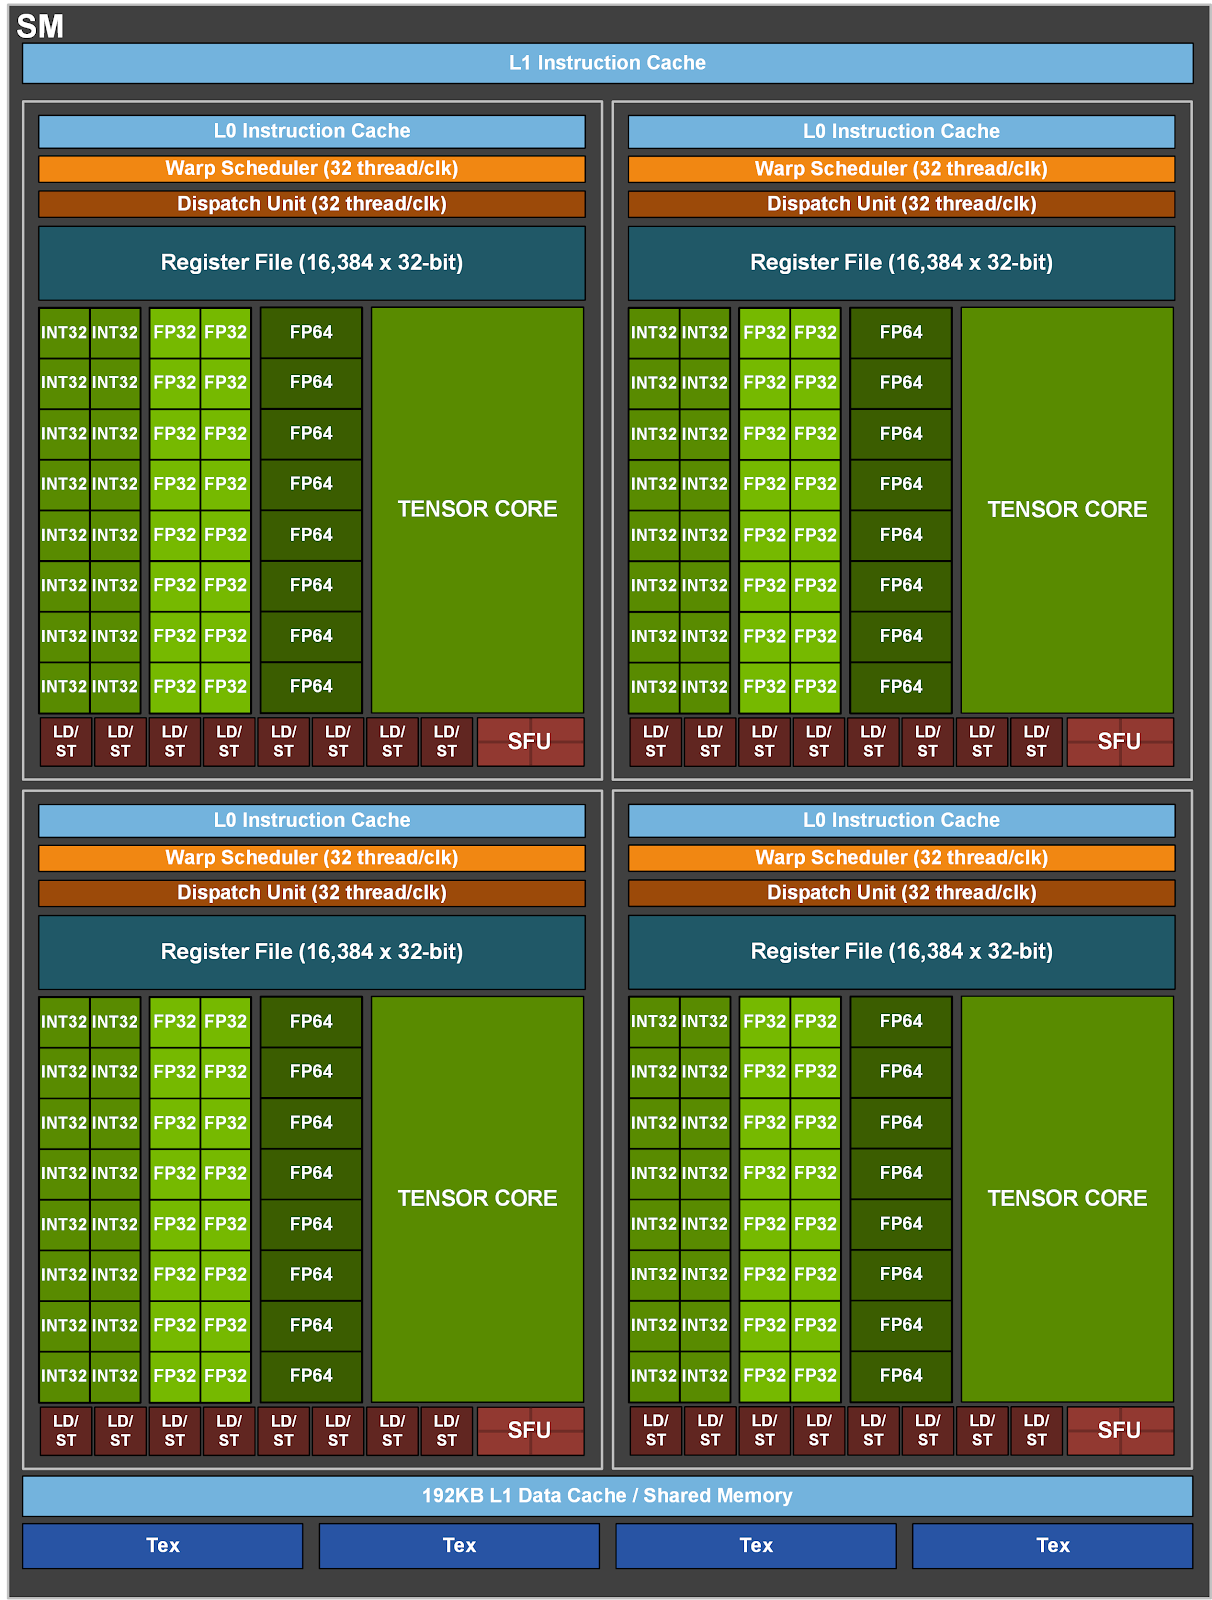
\includegraphics[scale=0.2]{gpu_new.png}
    \caption{GA100 streaming multiprocessor. The SM consists of 4 streaming processors (SP), which contains 16 FP32 Cores, 16 INT32 cores, 8 FP64 cores, and a single Tensor core. Furthermore, each SP has access to its own L0 instruction cache, warp scheduler, dispatch unit, and registers. On top of this, L0 instruction caches get the instructions from a shared L1 instruction cache. The data is accessed through a shared L1 cache. }
    \label{fig:gpu}
\end{figure}



\subsubsection{Warps and Thread Blocks}

To parallelize a calculation on a CPU, one would usually split the work into multiple threads. It works the same way in GPUs. GPUs spawn multiple threads, each doing a part of the work. These threads together are called a warp, as they execute the same instruction. This execution model is also called Single instruction, multiple threads (SIMT). The usual size of a warp is 32 threads.  Warps are the fundamental execution units in a GPU. Multiple warps constitute a thread block and several thread blocks are assigned on SMs. \cite{b2}


\begin{figure}[H]
    \centering
    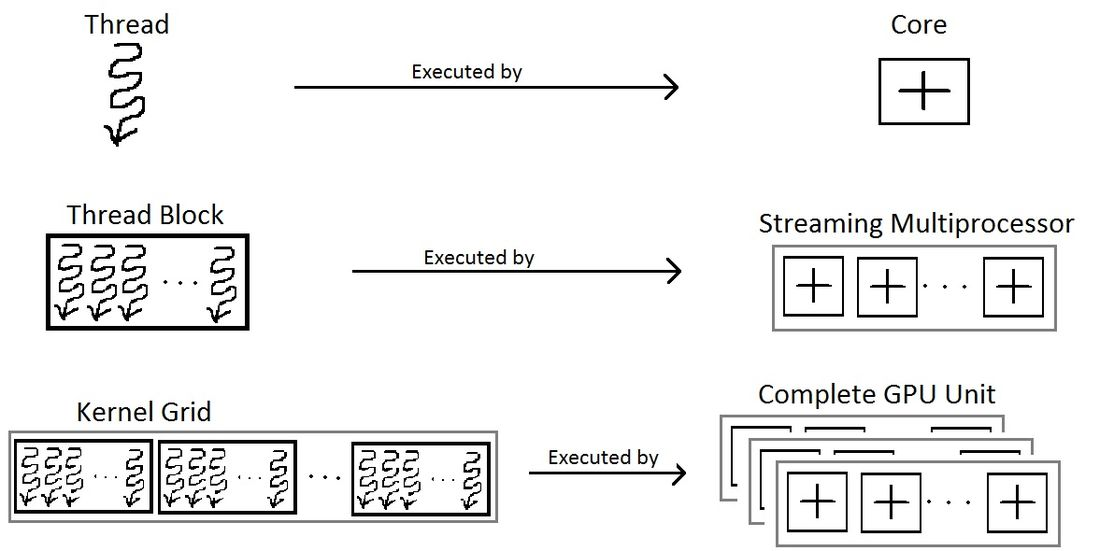
\includegraphics[scale=0.46]{kernel_grid.jpeg}
    \caption{Warps, Thread Blocks, Kernel Grids. The figure illustrates that threads are executed on cores, thread blocks on SMs, and kernel grids on GPUs.}
    \label{fig:enter-label}
\end{figure}

\subsubsection{Context Switching}
Contrary to the context switching in CPUs, where the current state of the thread, including registers values, program counter, etc. is saved to memory, the context switching between warps is much more efficient, since values are stored in register files in SM, hence consuming less time and energy. \cite{b2}
\subsubsection{Tensor Cores}


Tensor cores, seen in Figure 1, are compute cores designed for matrix multiplication. While multiplying matrices, one needs to store temporary values making it computationally intense. As operations like the following are used mainly for multiplying matrices,  r = (a * b) + c,  tensor cores are designed to accelerate it by making use of fused Multiply- add operation that performs floating-point multiply–add operation in one step, with a single rounding.  Therefore, it achieves higher performance and numerical precision. Another special point of tensor cores is their ability to compute mixed-precision calculations containing various datatypes eg. FP16, BF16, TF32, FP64, INT8, INT4. \ref{b18}


\subsubsection{Clock Speed}

CPUs are typically designed to boost clock speeds to multiple Gigahertz, prioritizing the execution of sequential calculations at a faster rate. In contrast, GPUs operate at clock speeds typically measured in the range of a few hundred megahertz. The reason for this is that increase in clock speed results in more power consumption, which in turn produces extreme heat in a small space. As it is hard to get rid of this heat efficiently with cooling devices, manufacturers opt to limit clock speed in megahertz. \cite{b17}

\subsubsection{Memory Bandwith}

GPUs make use of a memory technology called High Bandwith Memory that enables access speeds of a couple of hundred GB/s. Since GPUs only do basic arithmetic operations on data, there is a need to move big volumes of data from memory to the cores and from cores to memory. Contrary to GPUs, CPUs have to move data from RAM to caches to access.\cite{b17}

\begin{figure}[H]
    \centering
    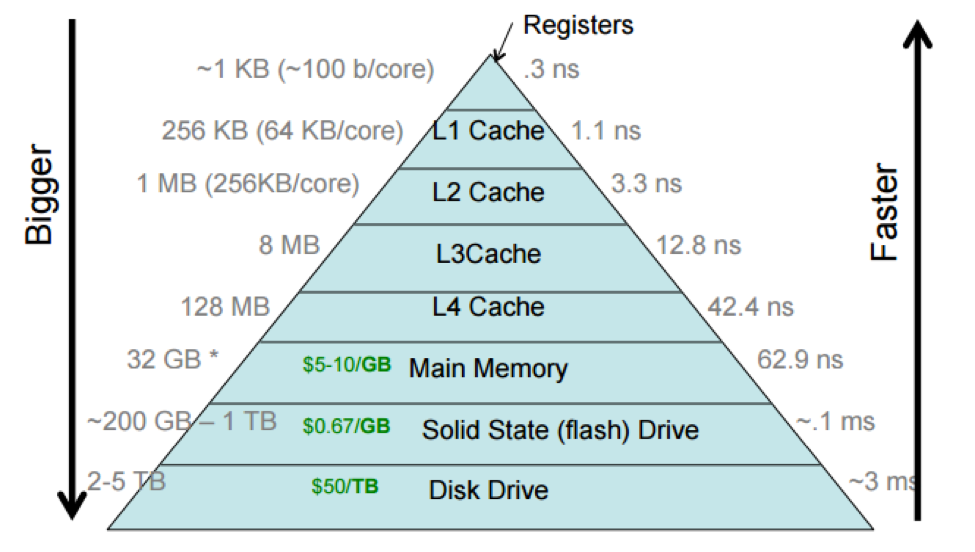
\includegraphics[scale=0.55]{l10-storage-hierarchy.png}
    \caption{The figure depicts a latency pyramid showcasing the hierarchy of caches and RAM. While the storage size gets bigger downwards, the access speed increases upwards.\cite{b24}}
    \label{fig:trad_2}
\end{figure} 

However, CPUs can impact computational performance badly when processing big amounts of data. Deep learning models, for instance, require a lot of memory to store model parameters and intermediate results, which can lead to frequent data transfers between main memory and cache, slowing down the overall computation.



\subsubsection{Core Count}


Most CPUs contain between 4 and 32 cores. However, GPUs have thousands of cores. Cpu cores are good at doing complex operations, but GPU cores are only suitable for basic operations
CPUs usually contain a small number of cores, ranging from around 4 to 32 cores. In contrast, GPUs boast an abundance of cores, often numbering in the thousands. While CPU cores excel at executing complex operations and handling a wide range of tasks, GPU cores are designed to handle simpler, more repetitive arithmetic operations. Therefore, it is easier to divide the work into thousands of pieces and distribute it onto the many cores in a GPU, which accelerate the computation a lot.
% \subsubsection{Power consumption}


\section{Using GPUs}
\subsection{Managing GPUs}
Since many users run their programs on HPCs, there is a need to regulate who can run where and how. Otherwise, the users would interfere with each other when they access the same GPU, which would waste time and energy, as some progress would be lost. One way to overcome this hurdle is Virtualization. In a CPU, one can figuratively give the same CPU to many users by isolating their access to it and dividing run-time. The same device virtualization can be used in GPUS, made possible by the CUDA wrapper library. It works by mapping virtual GPUs to physical GPUs, allowing extreme flexibility, since calculations could be moved from GPU to GPU. One way to illustrate this is the case when one uses GPU to the maximum and GPU heats up. The user can move his calculation to another fresh GPU and allocate a lightweight process to the heated GPU. \cite{b5}

\subsection{Securing GPUs}

It has been found that some applications may leave GPUs in an unstable state due to a bug in the driver. Furthermore, applications store data on GPUs, which needs to be cleaned up after the calculation is completed. Otherwise, it may allow the next user to access the previous user`s data, which is a major security breach. To counter this, a memory scrubbing method has been developed to fill the entire GPU memory with a pre-defined pattern.  \cite{b5}

\section{Programming on GPUs}
To accelerate calculations via GPUs, programmers need to use either GPU programming languages or toolkits. In this section, we will focus on low abstraction lightweight GPU programming toolkits such as CUDA and OpenCL, where developers need to write GPU kernels by themselves with no automatic code generation. To achieve efficient acceleration with GPUs, minimizing input/output (I/O) operations between the host and the GPU is crucial, otherwise, too much time would be lost with API calls between devices.
\subsection{CUDA}
Released in 2007 by Nvidia, CUDA is the most popular programming toolkit related to GPUs today. The compiler provided by CUDA supports an extended version of C that includes limited features from C++. It removes features such as recursive functions..., as these do not map to GPU hardware capabilities. The CUDA programming model concentrate on data parallelism and offers simplified programming tools to express kernels as a single thread of execution. This single thread expands into numerous threads that work together and share resources during execution. Furthermore, the CUDA compiler takes care of managing GPU kernel parameters, which are arguments passed on to a GPU kernel function to control its behavior or provide necessary data for computation. CUDA also provides various APIs for controlling the GPU. \cite{b3}



\begin{lstlisting}[language=C++, basicstyle=\ttfamily\small\lst@ifdisplaystyle\fontsize{8.9}{10.5}\fi
, caption=The function vectorAdd performs vector addition on the vectors A and B and stores the result in C. The arguments are given as pointers and the vector size is also supplied. \cite{b16}
,captionpos=b, label=lst:vector-add]
__global__ void vectorAdd( float *A,
float *B, float *C, int numElements) {
  int i;
  i = blockDim.x * blockIdx.x + threadIdx.x;
  if (i < numElements) {
    C[i] = A[i] + B[i];
  }
}
\end{lstlisting}

\begin{lstlisting}[label=lst:launch, basicstyle=\ttfamily\small, mathescape=true, captionpos=b, caption={This listing illustrates how a GPU kernel in CUDA can be started after configuring the kernel parameters.}]
int threadsPerBlock = 256;
int blocksPerGrid = (numElements +
threadsPerBlock - 1) / threadsPerBlock;
vectorAdd<<<blocksPerGrid, threadsPerBlock>>>
(d_A, d_B, d_C, numElements);
\end{lstlisting}
In Listing \ref{lst:vector-add}, we can see a basic CUDA code function that computes vector addition of A and B and stores the resulting vector in C. The index i has to be calculated with thread ID, since the code is designed to run in parallel on many cores. The keyword $ \_\_global $ defines a compute kernel. To demonstrate the configuration and launch of the above code, let's explore how it can be appropriately set up with the desired GPU kernel parameters and executed. The keyword \textlangle\textlangle\textlangle...\textrangle\textrangle\textrangle
 is used for assigning the number of cores. It configures 256 threads per block and sets the block count depending on the number of elements. Afterward, the kernel is called with the parameters and the code is executed on a GPU. \cite{b25}
 \vspace{\baselineskip}





\vspace{\baselineskip}


\subsection{OpenCL}
Focusing on portability, the OpenCL (Open Computing Language) library allows programmers to create code that runs on a variety of heterogeneous platforms, including CPUs, GPUs, and more. It offers a standardized interface for task- and data-based parallel computing. Contrary to CUDA, OpenCL is implemented as a library. Therefore, developers have to manage GPU resources on their own and process the input data to a suitable format for the GPU. Furthermore, developers do not need to modify the compilation process of the applications since openCL is just a library. An advantage of openCL is that GPU kernels aren't compiled with the rest of the application, but instead compiled at runtime by the openCL library. After the compilation of kernels, the application must manage them via the provided API. The kernels are written in OpenCL C/C++ languages.OpenCL C is based on the C99 standard and provides a C-like language and openCL C++ is based on openCL C and provides some extra C++ features as well. \cite{b4}

\begin{lstlisting}[language=C++, basicstyle=\ttfamily\small\lst@ifdisplaystyle\fontsize{8.9}{10.5}\fi
, caption=The function above calculates the dot product of a single row of a matrix A and a vector x:  \texttt{y_i = a_{i,:} \cdot x = \(\sum_{j} a_{i,j} x_{j}\)}
\cite{b4}
,captionpos=b]
__kernel void matvec(__global const float *A,
                     __global const float *x,
                    uint ncols,
                    __global float *y)
{

    size_t i = get_global_id(0);            
    __global float const *a = &A[i*ncols];    
    float sum = 0.f;                          
    for (size_t j = 0; j < ncols; j++) {
        sum += a[j] * x[j];
    }
    y[i] = sum;
}
\end{lstlisting}

The matvec function above illustrates some key elements from the OpenCL syntax. OpenCL C functions are marked $ \_\_kernel $ to signal that they are entry points into the program to be called from the host program. The keyword $ \_\_global $ indicates that the memory is shared among all processing elements (threads), albeit with high access latency. OpenCL offers more memory specifications such as $ \_\_local $ (shared by a group of threads), $ \_\_constant $ (writable by the host device and read-only for other devices) and $ \_\_private $ (accessible to a single thread only).\cite{b4}


\section{Performance Analysis}
As mentioned previously, GPUs excel at arithmetic calculations. In Figure
 \ref{fig:enter-label1},  a theoretical) performance comparison between CPUs and GPUs is depicted in GFLOPs. The X-axis represents the years from 2009 to 2015, with a two-year interval. On the Y-axis, the attainable GFLOPS is depicted, ranging from 0 to 11000 with a step size of 500. 
  The graph clearly illustrates that GPUs outperform CPUs in terms of computational power for floating-point calculations. Furthermore, CPUs can perform more double-precision calculations compared to single-precision calculations. However, GPUs calculate single precision operations better. What`s noteworthy is, that the gap between CPUs and GPUs continues to widen as the years progress. While CPU performance 
 grows linearly over time, GPU performance shows an almost exponential development over the same period. 


\begin{figure}[H]
    \centering
    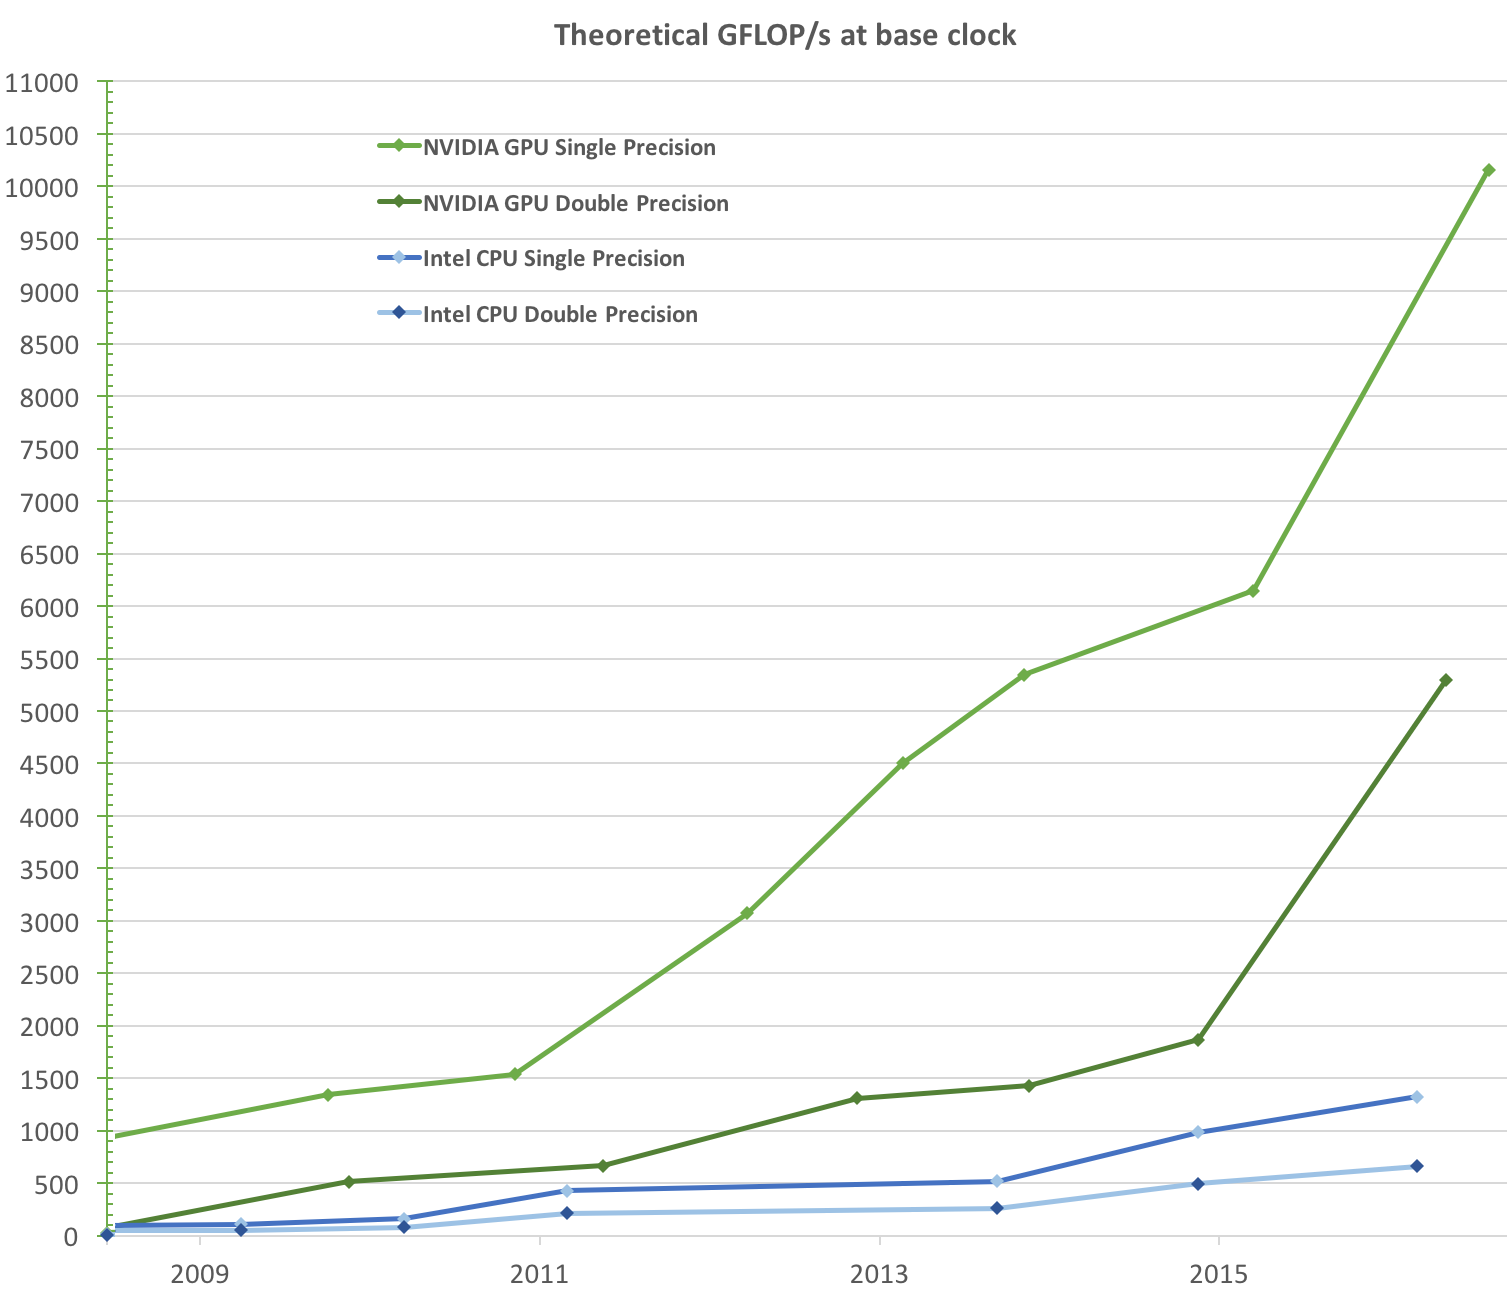
\includegraphics[scale=0.2]{PeakFlopsCPUGPU.png}
    \caption{The graph compares the floating-point performance of NVIDIA GPU and Intel CPU, each with single-precision and double-precision version. \cite{b22}}
    \label{fig:enter-label1}
\end{figure}







\section{Deep Learning}
\subsection{General information about deep learning}

To understand how deep learning can be accelerated by using GPUs it is important to know what deep learning is and how to separate it from neural networks and machine learning. “Artificial intelligence is the science and engineering of making intelligent machines, especially intelligent computer programs.”\cite{b8}. Machine learning is a part of artificial intelligence. It uses an algorithm to analyze and learn from data to make interpretations about this data. Basically, it describes a machine that gets trained by huge amounts of data. Deep learning is a part of machine learning and needs less direct human assistance to calculate results.\cite{b9}

\vspace{\baselineskip}
\subsection{Neural Networks}

Neural networks (NN) are used to implement deep learning. As shown in Figure \ref{fig:neural-network}, a NN has an input layer, at least one hidden layer, and one output layer and each layer consists of neurons. If a NN has more than one hidden layer it is called a deep neural network (DNN). Each neuron, also called node, is connected to other nodes from the next layer. Each layer has its own function to determine what to do with the input and each node has its own threshold value. When the calculated value from one specific node is above the threshold then this node is activated and the outcome is passed on to the nodes it is connected with from the next layer. If the node does not get activated no data flows from this node to other nodes. Each connection between the nodes has a weight. With these weights, the sent data gets updated and the new computed value is then used by the next node.\cite{b10}

\begin{figure}[H]
    \centering
    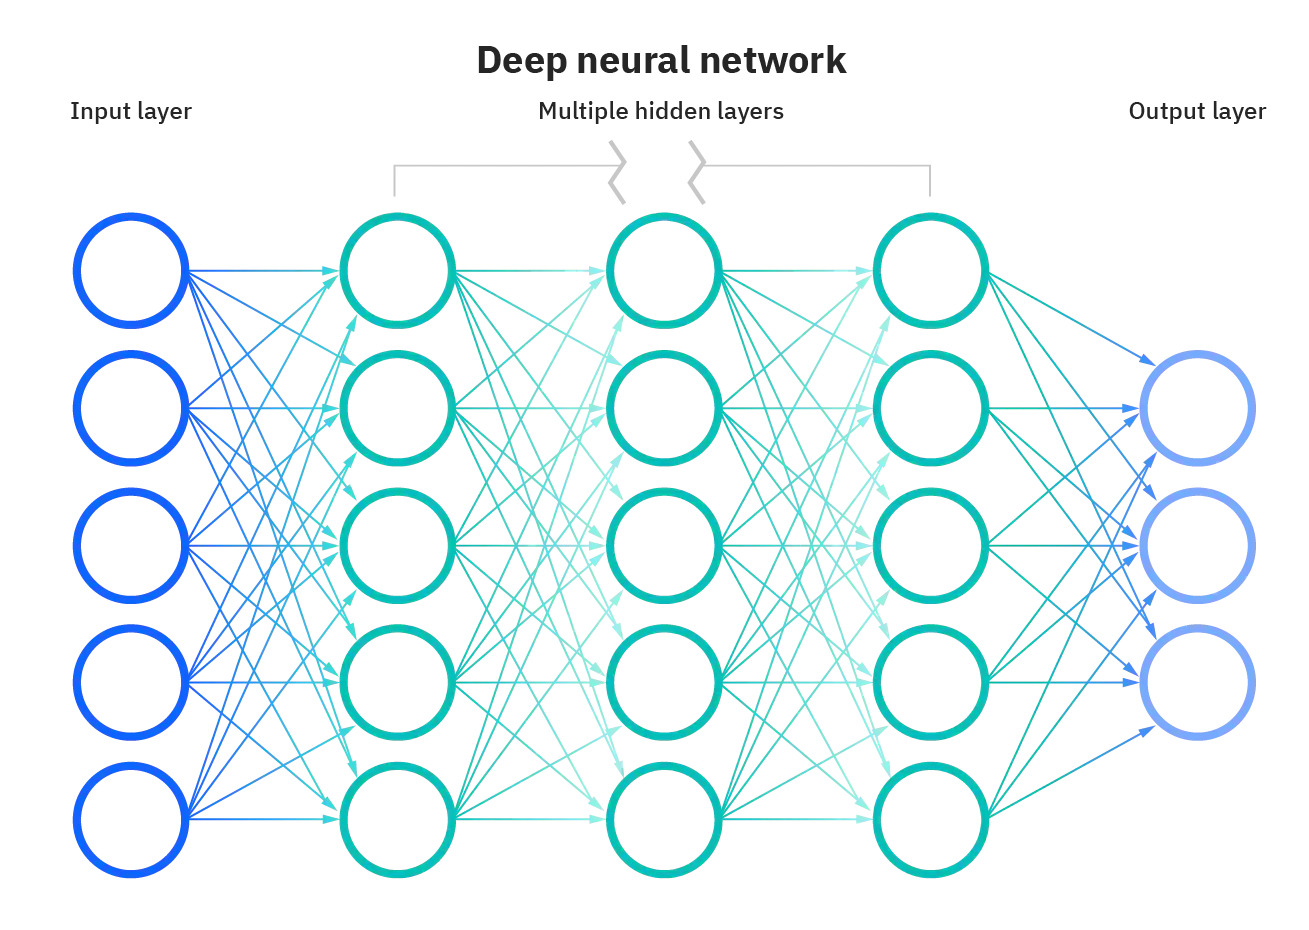
\includegraphics[scale=0.18]{NeuralNetwork.jpg}
    \caption{Deep neural network in which the circles represent the nodes and the arrows represent the connections between the nodes. \cite{b10}}
    \label{fig:neural-network}
\end{figure}

\subsection{DNN Training}

While training DNNs, data is given to the DNN and gets processed, most of the time, starting at the input layer until it reaches the output layer and creates an output, that means this data flows forward through the DNN. Now the calculated outcome can be compared to the expected outcome and an error will be computed. This phase is also called forward propagation. In the second phase, also called backward propagation, for each layer the gradients are computed which are then used to calculate the new weights. To optimize DNN models in terms of accuracy an algorithm called gradient descent or an algorithm similar to this one is normally used. This means that the DNN will make more accurate decisions by using this algorithm because the weights will be updated with this.\cite{b11}
DNNs are not the only type of neural network there are also for example convolutional neural networks (CNNs) or recurrent neural networks (RNNs). CNNs have high performance when it comes to image, speech or audio signal inputs. RNNs on the other hand are usually used for speech and language recognition.\cite{b9}

\vspace{\baselineskip}
\subsection{How are DNNs getting trained by using GPUs?}

Modern GPUs have a lot of computation power and are also often used in HPC systems to accelerate deep learning. One way to make the training for deep learning faster is to use distributed DNNs. This attempt uses workers that are running in parallel. There are many methods how distribute DNNs are being trained. We will look into how it is being done by using data parallelism. First, some data from the dataset needs to be loaded from the file system into the memory of the CPU. This random part of the dataset is called a mini-batch which is used to train the model. Then the CPU pre-processes the data so a GPU can fetch the data from the CPU memory. In the pre-processing, the CPU first prepares the data for the GPU and makes it accessible to the GPU in a ready queue. This method gives the DNN model, which is used, to all workers and splits the data, that is used to train the DNN, among the workers. Then each worker performs the forward as well as the backward propagation simultaneously and calculates the local gradients. These are called local because these are the gradients of each worker. But to update the weights of the NN these gradients need to be aggregated to global gradients. The new gradients are now distributed to all workers so that each worker can update their own model. To get all of the local gradients and aggregate them an implementation of the message passing interface (MPI) or more precisely the MPI Allreduce operation is used. Figure \ref{fig:trad_paralelism} presents how data parallelism can look like on two GPUs. In this Figure, the DNN model has just once been replicated because there are just two workers and one GPU is one worker.\cite{b11}

\begin{figure}[H]
    \centering
    \includegraphics[scale=0.46]{New_TraditionalDataParallelism.png}
    \caption{Traditional data parallelism model which is represents one way to accelerate DNN training in its basic steps with two GPUs. \cite{b11}}
    \label{fig:trad_paralelism}
\end{figure}

\vspace{\baselineskip}
\subsection{Optimization of the usual training method}

Because the GPUs are so powerful nowadays, they are not fully utilized with the data parallelism which is usually used. Researchers have recently presented a new method to get more performance out of each GPU. To accomplish that a tool called Multi-Process Service (MPS) from Nvidia is really useful. Basically, with this tool it is possible to run more than one of these processes on one worker or in this case GPU. This means that in Figure \ref{fig:trad_paralelism} on GPU 0 and GPU 1 the whole process, from loading the data to generating and distributing the global gradients, is duplicated. Each GPU still gets the same piece of data from the dataset but it will be divided into more pieces. In Figure \ref{fig:trad_paralelism}, the data that was being fetched was split into two mini-batches. Now the data will be split in so many mini-baches as processes run on each GPU times the number of GPUs that are used. This means that each process that runs at the same time on all the GPUs gets one mini-batch. The NN model gets still distributed to each GPU but these now need to replicate the model depending on how many processes run on the GPU. These have been the differences to the method before for each GPU. But because of the use of MPS, one more step is needed before data loading. In this step, a settings file is generated for every GPU so that MPS has all the necessary information and runs well.\cite{b11}

\vspace{\baselineskip}
\subsection{Tools that are used for training}

There are many tools that are there to use for deep learning and Horovod is one of them. It is an open-source framework which is often used for distributed deep learning and it supports many deep learning frameworks as well like PyTorch or TensorFlow. But this framework needs an MPI implementation. MPI is important to make the communication between GPUs, on the same node or on different nodes, and between MPS processes easier. Horovod is also useful because it is able to efficiently manage multiple GPUs whether they are on one or more machines. For the new method that researchers have recently developed Nvidia’s Multi-Process Service is needed to get more processes to run on a single GPU in parallel and it is still possible to use MPI. The processes that are running on a GPU have their own address space and depending on how much resources they need they can take some from each other if another process does not need them right now. Another reason why MPS is used is because usually, processes are not able to share the same physical resources in an efficient way. This is because GPUs are built so they would always have to switch contexts between the processes, which would be bad for performance, with MPS this problem is no longer there.\cite{b11}

\vspace{\baselineskip}
\subsection{Suitable hardware}

Because of the use of data parallelism to accelerate deep learning every new GPU with high amounts of cores and much memory is suitable for this task. In this case, the Nvidia A100 was used which has a lot of cores and memory. Some architectural differences of GPUs can also be useful to optimize performance. To use more than one GPU it is necessary to have connections between the devices like NVLink and InfiniBand. With this technology, multiple GPUs can be efficiently used in parallel.\cite{b11}

\section{Weather forecasting}
\subsection{Numerical Weather Prediction}
The main component to predict the weather is called numerical weather prediction (NWP). It is used all over the world and helps to predict the weather in our daily life and there are many different NWP models. NWP predicts future atmospheric conditions based on the current ones. These current conditions should be as accurate as possible to get a better outcome. It is also aware of physical processes and uses them to get accurate results.\cite{b12} To get more faster results high-performance systems and much parallelization are used.\cite{b13}

\vspace{\baselineskip}
\subsection{Weather Research and Forecasting}
The Weather Research and Forecasting (WRF) model is an NWP model and is usually used in scientific and operational areas. This model can be used for a lot of applications and is able to process data that is collected within a distance of some meters or many kilometers. It consists of many modules which were intended to run on CPUs. These different modules are more and more getting optimized to run on GPUs. To get a short insight on how these modules can be optimized we are focusing on the horizontal diffusion method.\cite{b13}

\vspace{\baselineskip}
\subsection{Horizontal diffusion method}
Some kind of diffusion is always part of every numerical weather model. This specific method is part of the advanced research version of WRF (WRF-ARW). The horizontal diffusion method is one of the methods of the WRF model which need a lot of computation power. It is used for example to manage numerical problems. Horizontal diffusion uses a three-dimensional grid for its calculations.\cite{b14}

\vspace{\baselineskip}
\subsection{How to accelerate the horizontal diffusion method with GPUs}
Because there already is an implementation for this method it first needs to be converted to code that GPUs can work with. In this case, Nvidia’s CUDA C has been used. While doing this it was important to use some guidelines to manage the GPUs memory and to manage some typical operations for GPU computations. The conversion to CUDA C was not that difficult because there was almost no effort to achieve united access to the data. To effectively optimize this method on GPUs their architecture needs to be taken into consideration. That means it is important to consider factors like memory access, utilization, etc.

The first optimization was done by increasing the GPU utilization. It was achieved by updating the thread block size. It is a simple but effective way to increase the performance.

The next acceleration has been accomplished by using the shared memory and L1 cache on GPUs which reduces the I/O latencies. Therefore, five of the most used 2D parameters such as 2D arrays are now moved to shared memory instead of moving them to global memory. It should be clear that shared memory is faster than global memory. For the GPU that was being used, there have been two different configuration modes and it has 64KB of on-chip memory in each SM. The first is named “preferL1” and the second one “prefershared”. With the first one, L1 will be 48KB, and the shared memory 16KB big. For the second one, it is the other way around. Because of the five 2D parameters just using 6.8KB of shared memory and the fact that a bigger cache increases the chance of getting a hit from the cached data higher the first configuration was used.

The last thing that was being done to increase the performance is to use compiler optimizations. Those are the use-fast-math-compiler and the O3 option when compiling. It needs to be said that these options affect the accuracy of the calculated mathematical results. But the impact on the output with and the output without these options was not that concerning.
From these three optimizations the first two had the most significant impact in increasing the performance.\cite{b14}


\vspace{\baselineskip}
\subsection{Possible performance gains with GPUs}
Horizontal diffusion was just one module of WRF. But how fast can WRF be when more modules are being accelerated? AceCAST is a recently developed software by TempoQuest that uses GPUs to accelerate the WRF model. It can perform high-resolution forecasts and provides a deeper view of upcoming weather phenomena. It is easily possible to use AceCAST with a usual WRF configuration because AceCAST uses a lot of the same modules as in WRF but is just refactored. It is also able to run on HPC systems and multi-node multi-GPU systems.

In the following, it will be analyzed how AceCAST performs on one node with multiple GPUs against one CPU node. The nodes are provided by the PARAM Siddhi-AI system. Each node consists of two 64 cores of AMD EPYC 7742 CPUs. It is worth mentioning that these CPUs have a bit more L3 cache than other CPU architectures typically have. The nodes with GPUs are additionally equipped with NVIDIAs A100 GPUs which have a great advantage over their predecessors, especially through the higher bandwidth of their memory. On the CPU-only node runs WRF 4.2.1 with all necessary tools and on the nodes with GPUs runs AceCAST. The input domains for this comparison are a small and a large one. The small input domain is called easter500 and consists of 12.7 million grid points and a 2 km resolution. The larger one is a user-defined input domain and covers four continents. It consists of 93.5 million grid points and has a 12 km resolution.

Figure \ref{fig:Perf_Graph_1} demonstrates the performance differences on different nodes with the easter500 as input. For this one already a single GPU accelerates the WRF model by 3.8 times compared to the CPU node. But the improvements by increasing the number of GPUs are getting less.

Figure \ref{fig:Perf_Graph_2} on the other hand shows the performance differences on different nodes with the larger user-defined input. With that, almost linear scalability can be observed when increasing the number of GPUs. The speed-up from 2 to 4 GPUs is about 1.7x and from 4 to 8 GPUs is also about 1.7x.

Overall, the GPU-accelerated WRF model (AceCAST) scales well with multiple GPUs. The significant speed-up from the CPU node to the GPU node is probably due to the better throughput of GPUs.\cite{b13}


\begin{figure}[H]
    \centering
    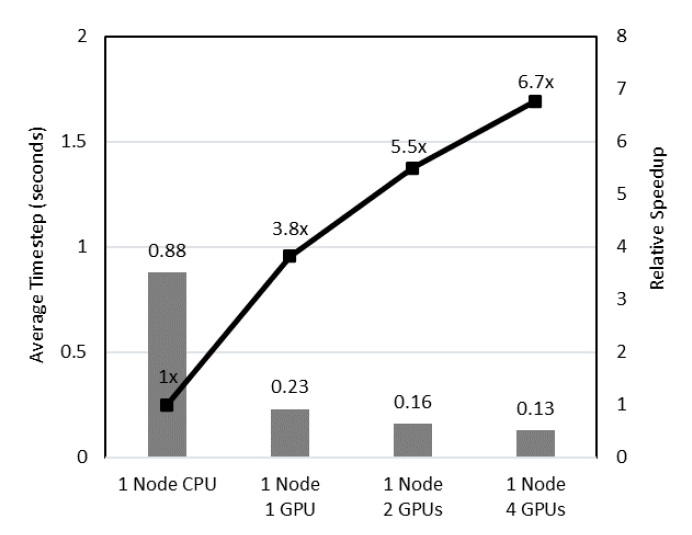
\includegraphics[scale=0.45]{Performance_one.png}
    \caption{Graph which shows the performance increase when using CPU nodes compared to nodes with GPUs. For the input domain easter500 was used with 2 KM resolution and 12.7 million gird points. \cite{b13}}
    \label{fig:Perf_Graph_1}
\end{figure}

\begin{figure}[H]
    \centering
    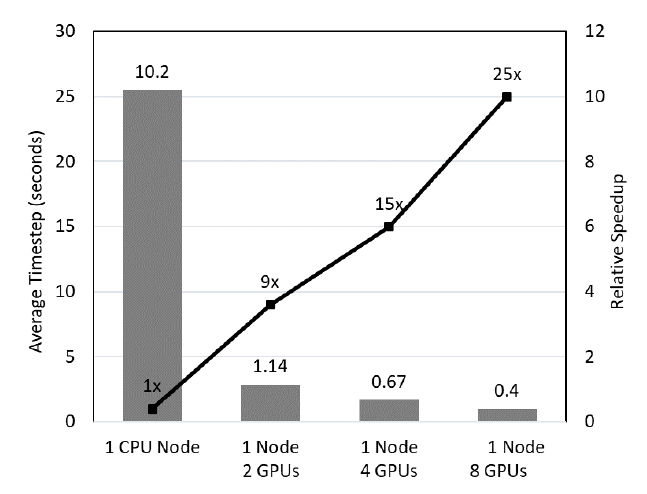
\includegraphics[scale=0.45]{Performance_two.png}
    \caption{Graph which represents the performance increase when using CPU nodes compared to nodes with GPUs. For the input domain user-defined input was used with 12 KM resolution and 93.5 million gird points. \cite{b13}}
    \label{fig:Perf_Graph_2}
\end{figure}


\section{Conclusion}
As we have seen with deep learning and weather forecasting, modern-day problems are quite complex and getting more complex day by day. From massive datasets in deep learning to short time constraints in weather forecasting, scaling CPUs with clusters was not a suitable solution for boosting performance effectively through scaling. Scientists turned to GPUs as accelerators, as they provided an immense number of compute cores for speed-up. GPUs can accelerate the weight calculations in Neural Networks by dividing the work into multiple subtasks and computing them concurrently. In weather forecasting, GPUs are helpful in accelerating many different tasks. For example, the WRF model which is used for weather forecasting can be sped up by accelerating its modules.



\begin{thebibliography}{00}
\bibitem{b1} "Graphics processing unit". Accessed on 08 June 2023. Available: \url{https://en.wikipedia.org/wiki/Graphics_processing_unit#Streaming_multiprocessor}

\bibitem{b2} "Thread block (CUDA programming)". Accessed on 08 June 2023. Available: \url{https://en.wikipedia.org/wiki/Thread_block_(CUDA_programming)}

\bibitem{b3} "CUDA". Accessed on 08 June 2023. Available: \url{https://en.wikipedia.org/wiki/CUDA}

\bibitem{b4} "OpenCL". Accessed on 08 June 2023. Available: \url{https://en.wikipedia.org/wiki/OpenCL}

\bibitem{b5} V. V. Kindratenko et al., "GPU clusters for high-performance computing," 2009 IEEE International Conference on Cluster Computing and Workshops, New Orleans, LA, USA, 2009, pp. 1-8, doi: 10.1109/CLUSTR.2009.5289128.



\bibitem{b6} "An illustration of a thread block from a software perspective", 21 September 2016, Author: Atshardul
\url{https://commons.wikimedia.org/wiki/File:Software-Perspective_for_thread_block.jpg}

\bibitem{b7} "Figure 5. The GA100 streaming multiprocessor (SM)",
\url{https://developer.nvidia.com/blog/nvidia-ampere-architecture-in-depth/}



\bibitem{b8} IBM, "What is artificial intelligence?" \url{https://www.ibm.com/topics/artificial-intelligence}

\bibitem{b9} IBM, "What is deep learning?" \url{https://www.ibm.com/topics/deep-learning}

\bibitem{b10} IBM, "What is a neural network?" \url{https://www.ibm.com/topics/neural-networks}

\bibitem{b11} N. Alnaasan, A. Jain, A. Shafi, H. Subramoni and D. K. Panda, "AccDP: Accelerated Data-Parallel Distributed DNN Training for Modern GPU-Based HPC Clusters," 2022 IEEE 29th International Conference on High Performance Computing, Data, and Analytics (HiPC), Bengaluru, India, 2022, pp. 32-41, \url{https://ieeexplore.ieee.org/document/10106337}

\bibitem{b12} Pu, Z., Kalnay, E. (2018). Numerical Weather Prediction Basics: Models, Numerical Methods, and Data Assimilation. In: Duan, Q., Pappenberger, F., Thielen, J., Wood, A., Cloke, H., Schaake, J. (eds) Handbook of Hydrometeorological Ensemble Forecasting. Springer, Berlin, Heidelberg. \url{https://doi.org/10.1007/978-3-642-40457-3_11-1}

\bibitem{b13} N. Agrawal, A. Das and M. Modani, "Scalability Analysis of Weather Research Forecast Model on NVIDIA Ampere based Dense GPU Cluster," 2022 International Conference on Computing, Communication, Security and Intelligent Systems (IC3SIS), Kochi, India, 2022, pp. 1-6, \url{https://ieeexplore.ieee.org/document/9885396}

\bibitem{b14} R. M. Gualán-Saavedra, L. D. Solano-Quinde and B. M. Bode, "GPU Acceleration of the Horizontal Diffusion Method in the Weather Research and Forecasting (WRF) Model," 2015 Asia-Pacific Conference on Computer Aided System Engineering, Quito, Ecuador, 2015, pp. 284-289, \url{https://ieeexplore.ieee.org/document/7287033}

\bibitem{b16} "CUDA Programming Model: A Code Example",
\url{https://www.run.ai/guides/nvidia-cuda-basics-and-best-practices/cuda-programming}
\bibitem{b17} "GPU MEMORY CLOCK SPEED VS GPU CORE CLOCK SPEED",
\url{https://vibox.co.uk/blog/gpu-memory-clock-speed-vs-gpu-core-clock-speed}

\bibitem{b18} "NVIDIA A100 Tensor Core GPU Architecture whitepaper",
\url{https://images.nvidia.com/aem-dam/en-zz/Solutions/data-center/nvidia-ampere-architecture-whitepaper.pdf}

\bibitem{b19} S. Ortiz, "What is ChatGPT and why does it matter? Here's what you need to know" \url{https://www.zdnet.com/article/what-is-chatgpt-and-why-does-it-matter-heres-everything-you-need-to-know/}

\bibitem{b20} J. Vincent "Meta’s powerful AI language model has leaked online — what happens now?" \url{https://www.theverge.com/2023/3/8/23629362/meta-ai-language-model-llama-leak-online-misuse}


\bibitem{b21} "Numerical weather prediction". Accessed on 24 June 2023. Available: \url{https://en.wikipedia.org/wiki/Numerical_weather_prediction}

\bibitem{b22} "Understanding GPU Architecture: Performance: GPU vs. CPU". Accessed on 24 June 2023. Available: \url{https://cvw.cac.cornell.edu/gpuarch/performance}

\bibitem{b23} "CPU vs. GPU: Making the Most of Both". Accessed on 24 June 2023. Available: \url{https://www.intel.com/content/www/us/en/products/docs/processors/cpu-vs-gpu.html}

\bibitem{b24} "Caching and the Storage Hierarchy". Accessed on 24 June 2023. Available: \url{https://cs.brown.edu/courses/csci0300/2021/notes/l09.html}
\bibitem{b25} "CUDA C++ Programming Guide". Accessed on 24 June 2023. Available: \url{https://docs.nvidia.com/cuda/cuda-c-programming-guide/index.html}
\bibitem{b26} "General-purpose computing on graphics processing units. Available: \url{https://en.wikipedia.org/wiki/General-purpose_computing_on_graphics_processing_units}




\end{thebibliography}

\end{document}
